\documentclass{beamer}
\usepackage[utf8]{inputenc}

\usetheme{Madrid}
\usecolortheme{default}
\usepackage{amsmath,amssymb,amsfonts,amsthm}
\usepackage{txfonts}
\usepackage{tkz-euclide}
\usepackage{listings}
\usepackage{adjustbox}
\usepackage{array}
\usepackage{tabularx}
\usepackage{gvv}
\usepackage{lmodern}
\usepackage{circuitikz}
\usepackage{tikz}
\usepackage{graphicx}

\setbeamertemplate{page number in head/foot}[totalframenumber]

\usepackage{tcolorbox}
\tcbuselibrary{minted,breakable,xparse,skins}



\definecolor{bg}{gray}{0.95}
\DeclareTCBListing{mintedbox}{O{}m!O{}}{%
  breakable=true,
  listing engine=minted,
  listing only,
  minted language=#2,
  minted style=default,
  minted options={%
    linenos,
    gobble=0,
    breaklines=true,
    breakafter=,,
    fontsize=\small,
    numbersep=8pt,
    #1},
  boxsep=0pt,
  left skip=0pt,
  right skip=0pt,
  left=25pt,
  right=0pt,
  top=3pt,
  bottom=3pt,
  arc=5pt,
  leftrule=0pt,
  rightrule=0pt,
  bottomrule=2pt,
  toprule=2pt,
  colback=bg,
  colframe=orange!70,
  enhanced,
  overlay={%
    \begin{tcbclipinterior}
    \fill[orange!20!white] (frame.south west) rectangle ([xshift=20pt]frame.north west);
    \end{tcbclipinterior}},
  #3,
}
\lstset{
    language=C,
    basicstyle=\ttfamily\small,
    keywordstyle=\color{blue},
    stringstyle=\color{orange},
    commentstyle=\color{green!60!black},
    numbers=left,
    numberstyle=\tiny\color{gray},
    breaklines=true,
    showstringspaces=false,
}
%------------------------------------------------------------
%This block of code defines the information to appear in the
%Title page
\title %optional
{4.11.21}
\date{October 3, 2025}
%\subtitle{A short story}

\author % (optional)
{Sai Hasini Pappula - EE25BTECH11044}

\begin{document}

%-----------------------------------
\begin{frame}
\titlepage
\end{frame}

%-----------------------------------
\begin{frame}{Question}
\begin{block}{Problem}
Find the equation of the plane passing through the line of intersection of:
\begin{align}
r \cdot (2\hat{i} + 2\hat{j} - 3\hat{k}) &= 7\\
r \cdot (2\hat{i} + 5\hat{j} + 3\hat{k}) &= 9 
\end{align}
such that the intercepts made by the plane on the $x$-axis and $z$-axis are equal.  
\end{block}
\end{frame}

%-----------------------------------
\begin{frame}{Solution}
Let the plane intercepts on $x$ and $z$ axes be equal.  
The $x$-intercept occurs when $y=0, z=0$ and the $z$-intercept occurs when $x=0, y=0$.  

This gives the system
\begin{align}
\begin{bmatrix}
2 + 2\lambda & 0 & 0 \\
0 & 0 & -3 + 3\lambda
\end{bmatrix}
\begin{bmatrix} x_0 \\ y_0 \\ z_0 \end{bmatrix} =
\begin{bmatrix} 7 + 9\lambda \\ 7 + 9\lambda \end{bmatrix}. 
\end{align}

Let coefficients be represented as:
\[
[a\ b\ c] = [2 + 2\lambda,\ 2 + 5\lambda,\ -3 + 3\lambda], \quad d = 7 + 9\lambda
\]
we can write:
\begin{align}
(2 + 2\lambda)x_0 = 7 + 9\lambda, \quad (-3 + 3\lambda) z_0 = 7 + 9\lambda. 
\end{align}
\end{frame}

%-----------------------------------
\begin{frame}{Solution}
Equal intercepts condition:
\begin{align}
x_0 = z_0 \quad \Rightarrow \quad 2 + 2\lambda = -3 + 3\lambda \quad \Rightarrow \quad \lambda = 5. 
\end{align}
Substitute in (4),
\begin{align}
a &= 2 + 2(5) = 12, \nonumber\\
b &= 2 + 5(5) = 27, \nonumber\\
c &= -3 + 3(5) = 12, \nonumber\\
d &= 7 + 9(5) = 52. 
\end{align}

\end{frame}

%-----------------------------------
\begin{frame}{Solution}
Substitute \(\lambda = 5\)
\begin{align}
\begin{bmatrix} a & b & c \end{bmatrix} = \begin{bmatrix} 2 + 10 & 2 + 25 & -3 + 15 \end{bmatrix} = \begin{bmatrix} 12 & 27 & 12 \end{bmatrix}, 
\end{align}
\quad    d = 7 + 45 = 52.
\\Hence, the required plane is:
\begin{align}
12x + 27y + 12z &= 52 
\end{align}
\end{frame}

%-----------------------------------
\begin{frame}[fragile]{C Code (1/2)}
\lstset{language=C}
\begin{lstlisting}
#include <stdio.h>

int main() {
    // Given plane coefficients
    float a1 = 2, b1 = 2, c1 = -3, d1 = 7;
    float a2 = 2, b2 = 5, c2 = 3, d2 = 9;
    
    float lambda; // scalar parameter
    // Step 1: Equal intercepts condition -> a/c must be same for x and z intercepts
    // From: (2 + 2λ)x = 7 + 9λ and (-3 + 3λ)z = 7 + 9λ, with x = z
    // => (2 + 2λ) = (-3 + 3λ)
    lambda = 5.0;
    // Step 2: Substitute λ = 5 in general plane coefficients
    float a = a1 + lambda * a2;  // 2 + 2λ
    float b = b1 + lambda * b2;  // 2 + 5λ
    float c = c1 + lambda * c2;  // -3 + 3λ
    float d = d1 + lambda * d2;  // 7 + 9λ
\end{lstlisting}
\end{frame}

\begin{frame}[fragile]{C Code (2/2)}
\lstset{language=C}
\begin{lstlisting}
    // Step 3: Display result
    printf("The required plane equation is:\n");
    printf("(%.0f)x + (%.0f)y + (%.0f)z = %.0f\n", a, b, c, d);

    // Optional: print intercepts for verification
    float x_intercept = d / a;
    float y_intercept = d / b;
    float z_intercept = d / c;
    
    printf("\nIntercepts on axes:\n");
    printf("x-intercept = %.2f\n", x_intercept);
    printf("y-intercept = %.2f\n", y_intercept);
    printf("z-intercept = %.2f\n", z_intercept);

    return 0;
}

\end{lstlisting}
\end{frame}

%-----------------------------------
\begin{frame}[fragile]{Python Code (1/3)}
\lstset{language=Python}
\begin{lstlisting}
import ctypes
import numpy as np
import matplotlib.pyplot as plt

# Load shared library
lib = ctypes.CDLL('./libplane.so')

# Define argument and return types
lib.find_plane.argtypes = [
    ctypes.c_float, ctypes.c_float, ctypes.c_float, ctypes.c_float,
    ctypes.c_float, ctypes.c_float, ctypes.c_float, ctypes.c_float,
    ctypes.POINTER(ctypes.c_float)
]
\end{lstlisting}
\end{frame}
\begin{frame}[fragile]{Python Code (2/3)}
\lstset{language=Python}
\begin{lstlisting}
# Input from user
print("Enter coefficients of Plane 1 (a1 b1 c1 d1): ")
a1, b1, c1, d1 = map(float, input().split())
print("Enter coefficients of Plane 2 (a2 b2 c2 d2): ")
a2, b2, c2, d2 = map(float, input().split())

# Output array
res = (ctypes.c_float * 5)()
lib.find_plane(a1, b1, c1, d1, a2, b2, c2, d2, res)

lam, a, b, c, d = [res[i] for i in range(5)]
print(f"\nλ = {lam:.2f}")
print(f"Required plane: {a:.2f}x + {b:.2f}y + {c:.2f}z = {d:.2f}")

# ---- Plotting Section ----
rng = np.linspace(-6, 6, 60)
X, Y = np.meshgrid(rng, rng)
\end{lstlisting}
\end{frame}
\begin{frame}[fragile]{Python Code (3/3)}
\lstset{language=Python}
\begin{lstlisting}
Z1 = (a1 * X + b1 * Y - d1) / (-c1)
Z2 = (a2 * X + b2 * Y - d2) / (-c2)
Z3 = (a * X + b * Y - d) / (-c)
fig = plt.figure(figsize=(10, 8))
ax = fig.add_subplot(111, projection='3d')
ax.plot_surface(X, Y, Z1, color='skyblue', alpha=0.5)
ax.plot_surface(X, Y, Z2, color='lightgreen', alpha=0.5)
ax.plot_surface(X, Y, Z3, color='salmon', alpha=0.6)

ax.set_xlabel('X-axis')
ax.set_ylabel('Y-axis')
ax.set_zlabel('Z-axis')
ax.set_title('Plane through Intersection (Equal X and Z Intercepts)')
ax.view_init(elev=28, azim=45)
plt.tight_layout()
plt.show()

\end{lstlisting}
\end{frame}

%-----------------------------------
\begin{frame}{Plot}
\begin{center}
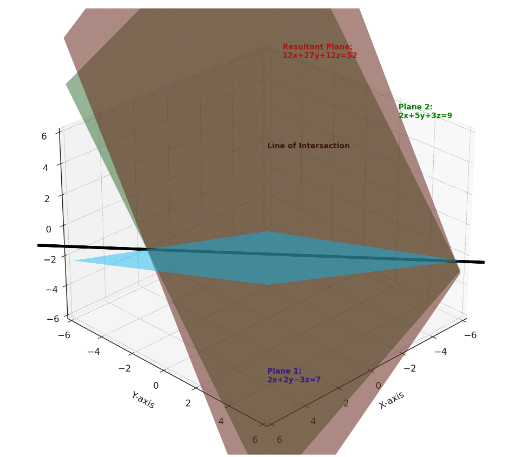
\includegraphics[width=0.7\columnwidth]{figs/plot8.png}
\end{center}
\end{frame}

\end{document}

